\section{Progress on the open problems}\label{pol:sec:progress}



\subsection{Problem \ref{pol:op:midpoint}: the even part and basepoint laws differ by an explicit factor}

\begin{theorem}\label{pol:thm:exact}
For every $\alpha>1/2$ and real $s\ge0$ put $R_\alpha(s)=\xi(\alpha-\sqrt s)/\xi(\alpha+\sqrt s)$. Then, unconditionally, $R_\alpha(0)=1$, $0<R_\alpha(s)<1$ for $s>0$, and
\begin{equation}\label{pol:eq:exact}
\begin{gathered}
\frac{\varphi^P_\alpha(s)}{\varphi^{(\alpha)}(s)}=\frac{2}{1+R_\alpha(s)},\\[4pt]
\psi^P_\alpha(s)-\psi_\alpha(s)=\log\frac{1+R_\alpha(s)}{2},
\end{gathered}
\end{equation}
where $\psi=-\log\varphi$ denotes the Laplace exponent, and for $s>0$ the difference of the exponents lies in $\left(-\log2,\,0\right)$. Hence $\varphi^{(\alpha)}\le\varphi^P_\alpha\le2\varphi^{(\alpha)}$ on $[0,\infty)$, and as $\alpha=\frac12+a\downarrow\frac12$,
\begin{equation}\label{pol:eq:rate}
\psi^P_\alpha(s)-\psi_\alpha(s)=-a\,\frac{\xi'}{\xi}\!\left(\tfrac12+\sqrt s\right)+O(a^2)
\end{equation}
locally uniformly in $s$. In particular $\varphi^P_\alpha\to\varphi$ and $\varphi^{(\alpha)}\to\varphi$ pointwise, so whenever the two families are laws they converge weakly to the reciprocal Xi law.
\end{theorem}

\begin{proof}
By definition $A_\alpha(\sqrt s)=\frac12\xi(\alpha+\sqrt s)\,(1+R_\alpha(s))$, which gives \eqref{pol:eq:exact}. For real $\sigma$, $\xi(\sigma)>0$, $\xi$ is symmetric about $\frac12$ and increasing on $[\frac12,\infty)$, because $\xi(\frac12+w)=\sum c_kw^{2k}$ with $c_k>0$. Since $\xi(\alpha-\sqrt s)=\xi(1-\alpha+\sqrt s)$ and $|\alpha+\sqrt s-\frac12|>|\frac12-\alpha+\sqrt s|$ when $\alpha>\frac12$ and $s>0$, we get $0<R_\alpha<1$ for $s>0$, while $R_\alpha(0)=1$. For \eqref{pol:eq:rate}, $\log R_\alpha(s)=\log\xi(\frac12+\sqrt s-a)-\log\xi(\frac12+\sqrt s+a)=-2a\frac{\xi'}{\xi}(\frac12+\sqrt s)+O(a^3)$, and $\log\frac{1+R}{2}=\frac12\log R+O((\log R)^2)$.
\end{proof}

Combined with Proposition~\ref{pol:prop:round}, Theorem~\ref{pol:thm:exact} evaluates the error of the midpoint rule exactly. For every $\alpha$ as in Proposition~\ref{pol:prop:round}, that is for $\alpha>\sigma_{\max}$ and unconditionally for $\alpha\ge1$, and every $s\ge0$,
\begin{equation}\label{pol:eq:midpoint}
\sum_{k\ge1}\log\!\left(1+\frac{s}{\tau_\alpha(k-\frac12)^2}\right)=\int_0^\infty\log\!\left(1+\frac{s}{\tau_\alpha(v)^2}\right)dv+\log\frac{1+R_\alpha(s)}{2}.
\end{equation}
The defect of the midpoint sum is a ratio of two values of $\xi$ on the real axis, and no modulus of continuity of the clock is needed. Numerically, for $\alpha=1,0.75,0.6,0.52$ the defect divided by $a=\alpha-\frac12$ varies by $1.2\%$ at $s=1$ and by $10\%$ at $s=100$, and approaches $-\frac{\xi'}{\xi}(\frac12+\sqrt s)=-0.0461,\,-0.408$, as \eqref{pol:eq:rate} predicts.

\subsection{Problem \ref{pol:op:pf2}: $f_X$ is log concave}

Write $N=f_Xf_X''-(f_X')^2$, so that PF$_2$ is $N<0$, and recall $\varphi(t^2)=\xi(\frac12)/\xi(\frac12+t)>0$ for real $t$.

\begin{lemma}[Origin]\label{pol:lem:origin}
$f_X'(0)=0$ and $f_X''(0)=-\frac1\pi\int_0^\infty t^2\varphi(t^2)\,dt<0$, so $f_X$ is log concave on a neighbourhood of $0$, unconditionally.
\end{lemma}

\begin{lemma}[Residue expansion]\label{pol:lem:residue}
Let $H=3\times10^{12}$ be the height up to which the zeros of $\xi$ are verified to be simple and on the critical line \cite{PT21}, let $0<T<H$ be different from every ordinate, and put $\eta_k=-\Xi(0)/\Xi'(\gamma_k)$. Then, unconditionally, for $x>0$,
\begin{equation}\label{pol:eq:residue}
\begin{gathered}
f_X(x)=\sum_{\gamma_k<T}\eta_k\,e^{-\gamma_kx}+E_T(x),\qquad \big|E_T^{(j)}(x)\big|\le C_j(T)\,e^{-Tx},\\[4pt]
C_j(T)=\frac{1}{2\pi}\int_{\mathbb R}\frac{|u-iT|^j\,\xi(\frac12)}{|\xi(\frac12+u-iT)|}\,du .
\end{gathered}
\end{equation}
The residues alternate in sign, $\eta_1>0>\eta_2$, and so on.
\end{lemma}

\begin{proof}
$f_X(x)=\frac1{2\pi}\int\varphi(t^2)e^{-itx}dt$. Move the line of integration to $\im t=-T$. The poles crossed are the zeros of $\xi(\frac12+t)$ with $-T<\im t<0$, which below $H$ are $t=-i\gamma_k$, simple; the vertical sides vanish because $|\xi(\sigma+i\tau)|$ grows like a gamma function as $|\sigma|\to\infty$, uniformly for bounded $\tau$. The residue at $-i\gamma_k$ is computed from $\xi'(\frac12-i\gamma)=i\,\Xi'(\gamma)$. The signs alternate because $\Xi$ changes sign at each simple real zero, starting from $\Xi(0)>0$.
\end{proof}

Numerically $\log|\eta_k|-\pi\gamma_k/4$ equals $-5.2,-8.0,-8.8,-9.7,-11.1$ for $k=1,10,20,40,60$, so $|\eta_k|$ grows like $e^{\pi\gamma_k/4}$ up to a power of $\gamma_k$, and the expansion is useful only for $x>\pi/4$.

\begin{lemma}[Two exponentials]\label{pol:lem:two}
If $f=Ae^{-ax}+Be^{-bx}$, then $ff''-(f')^2=AB\,(b-a)^2e^{-(a+b)x}$. With $A=\eta_1>0>B=\eta_2$ this is negative.
\end{lemma}

The proof is a one line expansion. With $T=23$, between $\gamma_2$ and $\gamma_3$, Lemmas~\ref{pol:lem:residue} and \ref{pol:lem:two} give $Ne^{(\gamma_1+\gamma_2)x}=\eta_1\eta_2(\gamma_2-\gamma_1)^2+\varepsilon(x)$, where $|\varepsilon(x)|$ is bounded by a sum of terms each decreasing in $x$, built from $C_0,C_1,C_2$ and $|\eta_1|,|\eta_2|$. Numerically $\eta_1=359.524$, $\eta_2=-28007.2$, $\eta_1\eta_2(\gamma_2-\gamma_1)^2=-4.776\times10^{8}$, and $C_0,C_1,C_2=5.99\times10^4,\ 1.38\times10^6,\ 3.19\times10^7$.

\begin{theorem}[PF$_2$, floating point certificate]\label{pol:thm:pf2}
The density $f_X$ of $X=Z\sqrt{2Y}$ is log concave on $\mathbb R$. The certificate has three parts, for $x\ge0$ (the density is even).
\begin{enumerate}
\item[(A)] On $[0,0.95]$, direct quadrature of $f^{(j)}(x)=\frac1\pi\int_0^\infty\varphi(t^2)\frac{d^j}{dx^j}\cos(tx)\,dt$ at the left end $x_i$ of each of $770$ cells, with $\sup|N'|$ on a cell of length $h$ bounded by $B(h)$ through $|f^{(j)}(y)|\le|f^{(j)}(x_i)|+h\,m_{j+1}$ and $m_j=\frac1\pi\int_0^\infty t^j\varphi(t^2)dt$ ($m_0,\dots,m_4=1.899,\ 7.321,\ 44.94,\ 355.8,\ 3361$), proves $N<0$. The cells are chosen from the left, each as long as possible with $h\,B(h)\le0.99\,|N(x_i)|$, so that $N\le N(x_i)+h\,B(h)<0$ on the cell; any factor in $(0,1)$ in place of $0.99$ works ($814$ cells at $0.9$, $1165$ at $0.5$).
\item[(B)] On $[0.95,2.1]$, the expansion \eqref{pol:eq:residue} with the first twelve zeros and $T=\frac12(\gamma_{12}+\gamma_{13})=57.90$ gives $Ne^{(\gamma_1+\gamma_2)x}$ as an explicit exponential sum plus a remainder with decreasing majorant; $26$ equal cells certify negativity ($22$ equal cells are the least that do, and two adaptive cells suffice). At $x=0.95$ the sum is $-2.18\times10^8$ and the remainder at most $7.03\times10^6$.
\item[(C)] For $x\ge2.1$ the two term form with $T=23$ has $|\varepsilon(x)|\le4.687\times10^8<4.776\times10^8$: the majorant decreases and equals $4.687\times10^8$ at $x=2.1$.
\end{enumerate}
\end{theorem}

Figure~\ref{pol:fig:two} (left) shows $-(\log f_X)''$. It is $23.66$ at the origin and then decays like $\frac{|\eta_2|}{\eta_1}(\gamma_2-\gamma_1)^2e^{-(\gamma_2-\gamma_1)x}$, which is $4.0\times10^{-9}$ at $x=4$: the log concavity of the tail is exponentially thin, and it is held up by the sign of $\eta_2$ alone.

\begin{figure}[ht]
\centering
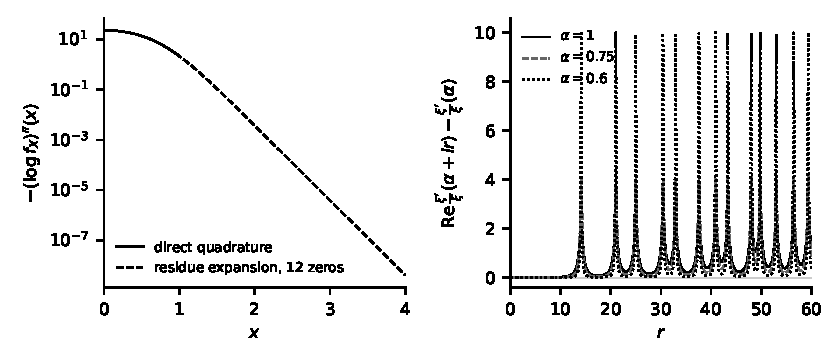
\includegraphics[width=\textwidth]{fig/polya_fig2.pdf}
\caption{Left: $-(\log f_X)''(x)$ on a log scale, from direct quadrature on $[0,0.95]$ (solid) and from the residue expansion with twelve zeros on $[0.95,4]$ (dashed); it is positive throughout, which is Theorem~\ref{pol:thm:pf2}. Right: the compensated clock condition $D_\alpha(r)=\re\frac{\xi'}{\xi}(\alpha+ir)-\frac{\xi'}{\xi}(\alpha)\ge0$ of Theorem~\ref{pol:thm:exactlemma} for $\alpha=1$ (solid), $0.75$ (dashed) and $0.6$ (dotted), computed from the Hadamard sum over the first $1700$ zeros at step $0.02$; $D_\alpha$ vanishes at $r=0$ and is positive after, with a peak of height about $1/(\alpha-\frac12)$ at each ordinate. Drawn by \texttt{polya\_fig.py}.}\label{pol:fig:two}
\end{figure}

\paragraph{Numerics.} The certificate is reproduced by \texttt{code/polya\_density.py} (\texttt{code/\allowbreak README.md}) in mpmath at 80 digits. The values $f_X^{(j)}$ on $[0,1.6]$ come from composite Gauss Legendre quadrature and beyond $1.6$ from the residue expansion; the two agree to a relative $2\times10^{-20}$ at $x=1.6$ with fourteen zeros and to $8\times10^{-42}$ with forty (for the derivatives of orders one to three, to $2\times10^{-18}$ and $6\times10^{-39}$). The quadrature errors are many orders of magnitude below the margins of Parts (A) and (B). Part (C) is thin: the majorant falls below $4.776\times10^8$ from $x=2.0904$ on, so that at $x=2.1$ the margin is $1.9\%$ of the bound, and a relative error of $2\%$ in $C_0,C_1,C_2$ would break it; the constants are stable to many digits under two quadrature layouts. The only arithmetic input is that the first thirteen zeros are simple and on the line.

The mechanism of Lemma~\ref{pol:lem:two} extends, as a sketch, to every order $n$ with $\gamma_n<H$ in the far tail. If $x_1<\dots<x_n$, $y_1<\dots<y_n$ and every $x_i-y_j$ is large, the Cauchy Binet expansion of $\det[f_X(x_i-y_j)]$ is dominated by the term from $\gamma_1,\dots,\gamma_n$, whose sign is $\operatorname{sgn}(\eta_1\cdots\eta_n)\,(-1)^{n(n-1)/2}=(-1)^{\lfloor n/2\rfloor+n(n-1)/2}=+1$. So the PF$_n$ minors with $\gamma_n<H$ are positive far in the tail, unconditionally, provided the remainder $E_T$ of \eqref{pol:eq:residue}, which is not a sum of exponentials, can be dominated inside the determinant; Proposition~\ref{pol:prop:hankel} does this for coalescing points.

\begin{theorem}[$f_X$ is uniformly close to a PF$_\infty$ density]\label{pol:thm:approxpf}
Let $X_{\mathrm{on}}=\sum L_\gamma/\gamma$, the sum over the zeros on the critical line with independent standard Laplace variables. Unconditionally $X_{\mathrm{on}}$ has a PF$_\infty$ density $f_{\mathrm{on}}$, and for $j=0,1,2$
\begin{equation}\label{pol:eq:approxpf}
\sup_x\big|f_X^{(j)}(x)-f_{\mathrm{on}}^{(j)}(x)\big|\le\varepsilon_j:=\frac{1}{\pi}\int_0^\infty t^j\,\Pi_K(t)\left(2S\,t^2+S^2t^4\right)dt,
\end{equation}
where $\Pi_K(t)=\prod_{k\le K}(1+t^2/\gamma_k^2)^{-1}$ for any $K$ with $\gamma_K<H$, and $S=\sum_{\gamma>H}\gamma^{-2}\le(\log\frac{H}{2\pi}+2)/(2\pi H)=1.533\times10^{-12}$ for $H=3\times10^{12}$. With $K=300$, $\varepsilon_0\le1.57\times10^{-10}$, $\varepsilon_1\le1.3\times10^{-9}$ and $\varepsilon_2\le1.3\times10^{-8}$. Consequently every $n\times n$ minor $\det[f_X(x_i-y_j)]$ with ordered $x$ and $y$ is at least $-n\cdot n!\,(2\varepsilon_0+f_{\mathrm{on}}(0))^{n-1}\varepsilon_0$, which is $-1.1\times10^{-8}$ for $n=3$ and $-1.2\times10^{-7}$ for $n=4$, since $f_{\mathrm{on}}(0)\le\frac1\pi\int_0^\infty\Pi_K=1.976$.
\end{theorem}

\begin{proof}
The characteristic function of $X_{\mathrm{on}}$ is $\varphi_{\mathrm{on}}(t^2)=\prod_{\text{on line}}(1+t^2/\gamma^2)^{-1}$, the reciprocal of a function of type \eqref{pol:eq:LP}, so $f_{\mathrm{on}}$ is PF$_\infty$ by Schoenberg's theorem whatever the zeros off the line do. Write $\varphi(t^2)=\varphi_{\mathrm{on}}(t^2)R(t^2)$, where $R$ collects the off line zeros. Each conjugate pair $s_\rho,\bar s_\rho$ with $s_\rho=-a^2$, $a=\gamma-i\delta$, contributes $1/P_\rho(t^2)$ with $P_\rho(v)=1+2v\re(a^{-2})+v^2|a|^{-4}$. Since $\gamma>H>\frac12>|\delta|$, $\re a^{-2}=(\gamma^2-\delta^2)/|a|^4>0$, so $P_\rho\ge1$ on $[0,\infty)$, $0<R\le1$ and $1-R\le\sum_\rho(P_\rho-1)\le2St^2+S^2t^4$. Fourier inversion gives $|f_X^{(j)}-f_{\mathrm{on}}^{(j)}|\le\frac1\pi\int_0^\infty t^j\varphi_{\mathrm{on}}(t^2)(1-R(t^2))\,dt$, and $\varphi_{\mathrm{on}}\le\Pi_K$ because the first $K$ zeros are on the line. The tail sum $S$ follows by partial summation from the zero counting formula with an explicit error term \cite{HSW22}; Proposition~\ref{mw:prop:approx} gives the sharper value $1.4798\times10^{-12}$ for the same sum, and the constants of the theorem were computed with the larger one. For the minors, expand the determinant multilinearly in the differences $f_X-f_{\mathrm{on}}$ and use $\det[f_{\mathrm{on}}(x_i-y_j)]\ge0$ and $|f_{\mathrm{on}}|\le f_{\mathrm{on}}(0)$.
\end{proof}

RH is the statement that the uniform distance of $f_X$ to a PF$_\infty$ density is zero. The bound on the minors grows quickly with $n$ (it exceeds $1$ at $n=10$), so for large orders the theorem gives no information, and a failure of PF$_3$ would be invisible at the level $10^{-8}$. Numerically there is none: over $6050$ Toeplitz type minors for each of $n=3$ and $n=4$, with spacings $0.02d$ and $0.02(d+1)$, $1\le d\le25$, and offsets up to $1.2$, all are positive and the smallest normalised minor $\det[f_X(x_i-y_j)]/\prod_if_X(x_i-y_i)$ is $1.6\times10^{-10}$ for $n=3$ and $3.5\times10^{-19}$ for $n=4$. Both occur at the smallest spacing; most of the smallness comes from nearly coinciding points, since for $n=3$ the smallest value over the offsets grows with $d$ from $1.6\times10^{-10}$ at $d=1$ to $6.0\times10^{-2}$ at $d=25$.
